\documentclass[12pt]{article}
\usepackage[margin=1in]{geometry}
\usepackage{amsmath,amsthm,amssymb,amsfonts}
\usepackage{graphicx}

\newcommand{\N}{\mathbb{N}}
\newcommand{\Z}{\mathbb{Z}}
\newcommand{\unit}[1]{\ensuremath{\, \mathrm{#1}}}

\newenvironment{problem}[2][Problem]{\begin{trivlist}
\item[\hskip \labelsep {\bfseries #1}\hskip \labelsep {\bfseries #2.}]}{\end{trivlist}}
%If you want to title your bold things something different just make another thing exactly like this but replace "problem" with the name of the thing you want, like theorem or lemma or whatever

\newenvironment{answer}[2][Answer]{\begin{trivlist}
\item[\hskip \labelsep {\bfseries #1}\hskip \labelsep {\bfseries #2.}]}{\end{trivlist}}

\begin{document}

%\renewcommand{\qedsymbol}{\filledbox}
%Good resources for looking up how to do stuff:
%Binary operators: http://www.access2science.com/latex/Binary.html
%General help: http://en.wikibooks.org/wiki/LaTeX/Mathematics
%Or just google stuff

\title{AST 231: Problem Set 1}
\author{Jonas Powell}
\maketitle

\begin{problem}{1}
The Solar Constant is about 1365 W/m$^2$. Calculate the distance from a 100 W light bulb at which its flux has the same value as the Solar Constant. Verify your result by holding your hand at that distance from the light bulb, but PLEASE do not BURN yourself due to an incorrect calculation!
\end{problem}

\begin{answer}{1}

  Recognizing that the Solar Constant, $SC=1365 \frac{W}{m^{2}}$, is an energy scaled by the area receiving that energy (i.e. a flux), we can equate that flux received to the flux received from a $ 100 W $ lightbulb and solve for the distance at which the fluxes are the same.

  \begin{equation}
    1365 \frac{W}{m^{2}} = \frac{100}{4 \pi r^{2}} \frac{W}{m^{2}}
  \end{equation}
  \\

  With some simple rearranging, we find that:
  \\

  \begin{equation}
    \begin{align}
      r & = \sqrt{\frac{100}{1365 * 4 \pi}} \\
      & = 0.076 \text{ meters} \\
      & \approx 3 \text{ inches}
    \end{align}
  \end{equation}

\end{answer}

\bigskip
\bigskip


\begin{problem}{2}
A star that appeared to be single was measured to have V = 12.13 and B-V = 1.28. On closer inspection with HST it was found that this star is actually a visual binary, with component B being 0.90 mag fainter in V and 1.80 mag fainter in B than component A. Calculate the V magnitude and B-V color of each component.
\end{problem}

\begin{answer}{2}

  We begin with the given equation relating a difference in magnitudes of two sources to the ratio of their fluxes:

  \begin{equation}
    M_{1} - M_{2} = -2.5 \log{\frac{f_{\nu,1}}{f_{\nu,2}}}
  \end{equation}

  We can also note that the magnitude in a certain band (V, for example) of a source can be related to the source's flux using the band's zero-point flux as:

  \begin{equation}
    V_{source} = -2.5 \log{\frac{f_{source, V-band}}{\text{zero point flux (V-band)} = 3781}}
  \end{equation}

  We are given the difference in magnitudes of each source, A and B, for the B and V bands:

  \begin{equation}
    V_{B} - V_{A} = 0.90
  \end{equation}
  \begin{equation}
    B_{B} - B_{A} = 1.80
  \end{equation}

  Likewise, we are given the two objects' total V-band magnitude and their B-V color, allowing us to find the B-band magnitude:
  \begin{equation}
    V_{Tot} = 12.13
  \end{equation}
  \begin{equation}
    B_{Tot} - V_{Tot} = 1.28
  \end{equation}
  \begin{equation}
    B_{Tot} = 1.28 + V_{Tot} = 13.41
  \end{equation}


  Combining (3) and (5) we can find the sources' V-band flux ratio:

  \begin{equation}
    V_{A} - V_{B} = 0.90 = -2.5 \log{\frac{f_{V,A}}{f_{V,B}}} \\
  \end{equation}

  %\begin{equation}
  $$  \rightarrow \frac{f_{V,A}}{f_{V,B}} = 10^{\frac{-0.90}{2.5}} \\ $$
  %\end{equation}

  %\begin{equation}
    $$ \rightarrow f_{V,B} = 0.44 * f_{V,A} $$
  %\end{equation}

  \begin{equation}
    f_{V, Tot} = 1.44 * f_{V,A}
  \end{equation}




  Drawing on (4) and (7), we can now draw out the total flux for the two sources. Using that, we draw out the two individual fluxes in non-relative terms.

  %\begin{equation}
  $$  V_{Total}  = 12.13  = -2.5 \log{\frac{f_{V, Tot}}{3781}} \\
               = -2.5 \log{\frac{1.44 * f_{V,A}}{3781}} $$
  %\end{equation}

  \begin{equation}
    \begin{align}
    f_{V,A} & = \frac{3781}{1.44} * 1.4 * 10^{-5} \\
            & = 0.037
    \end{align}
  \end{equation}

  \begin{equation}
    \begin{align}
      f_{V,B} & = 0.44 * f_{V,A} \\
              & = 0.016
    \end{align}
  \end{equation}

  We can follow a similar process to find the B-band fluxes.

  \begin{equation}
    B_{A} - B_{B} = 1.80 = -2.5 \log{\frac{f_{B,A}}{f_{B,B}}} \\
  \end{equation}

  %\begin{equation}
    $$ \rightarrow \frac{f_{B,A}}{f_{B,B}} = 10^{\frac{-1.80}{2.5}} $$
  %\end{equation}

  % \begin{equation}
  $$ \rightarrow f_{B,B} = 0.19 * f_{B,A} $$
  % \end{equation}

  \begin{equation}
    f_{B, Tot} = 1.19 * f_{B,A}
  \end{equation}


  Following information from http://www.adamgginsburg.com/filtersets.htm, we find that the zero-point flux for the B-band is 4130.

  %\begin{equation}
  $$ B_{Total} = 13.41 = -2.5 \log{\frac{f_{B,Tot}}{4130}} \\
              = -2.5 \log{\frac{1.44 * f_{B,A}}{4130}}  $$
  %\end{equation}

  \begin{equation}
    \begin{align}
    f_{B,A} & = \frac{4130}{1.19} * 4.325 * 10^{-6}
            & = 0.015
    \end{align}
  \end{equation}

  \begin{equation}
    \begin{align}
      f_{B,B} & = 0.19 * f_{B,A}
              & = 0.00285
    \end{align}
  \end{equation}


  Now that we have both objects' individual fluxes, we can draw again on (4) to get each source's individual B and V magnitudes, then subtract each source's V magnitude from its B magnitude to get the final table of desired values.


  \bigskip
  \bigskip

  \centering
  \begin{tabular} {cccccc}
  Source Name & B-Magnitude     & V-Magnitude   & B-V   \\
  \hline
  \hline
  Source A    & 15.40           & 12.52         & 2.88 \\
  Source B    & 13.59           & 13.43         & 0.16  \\
  \hline

  \end{tabular}

\end{answer}


\bigskip
\bigskip






\begin{problem}{3}
Photometric data on a star are given in the table below. For your convenience, I also provide the flux density of a zero magnitude star and effective wavelengths of the filters for the photometric system in which the star was observed. The flux densities are in Jansky's (Jy), a favorite unit of infrared and radio astronomers. Be careful, because the Jy is a unit of F$_\nu$, not F$_\lambda$. There is a link on the course Moodle page to a Web site that will help you do the conversions correctly. Plot the tabulated data on a $F_\lambda$ versus log ($\lambda$) diagram. Make the scale be W/m$^2$/micron, as on the example, with wavelength expressed in microns. On the same diagram plot the blackbody curve (Planck function) with the temperature that you think best fits the data. In other words, you are using the spectral energy distribution (fondly called the SED by most astronomers) to estimate the effective temperature of the star. Be sure to state the effective temperature that you derive for the star by this method.
\bigskip
\smallskip

\begin{tabular} {cccccc}

Filter & V & I & J & H & K \\
\hline
\hline
Magnitude & 16.11 & 14.47 & 13.42 & 12.74 & 12.47 \\
Effective Wavelength (in microns) & 0.545 & 0.798 & 1.25 & 1.65 & 2.20 \\
Zero mag Flux Density (Jy) & 3636.0 & 2416.0 & 1670.0 & 980.0 & 620.0 \\
\hline

\end{tabular}

\end{problem}


\begin{answer}{3}

Since we would like to convert the given magnitudes into fluxes to plot against a blackbody curve, we must again massage (4) to find our flux.

\begin{equation}
  f_{\nu} = \text{Zero Point Flux (Jy)} * 10^{-\text{Magnitude}/2.5}
\end{equation}

We would rather have our fluxes be in terms of wavelength, $\lambda$, than frequency. From the Spitzer website linked on the Moodle page, we learn that:
\begin{equation}
  F_{\lambda} = F_{\nu} * 10^{-26} * \frac{c}{\lambda^{2}}
\end{equation}

With our data now in the appropriate form, we would like to fit a blackbody curve to them. Since the Planck function's form is controlled by temperature, a good fit will tell us the source's temperature. As above, we would like this model to be a function of wavelength, so we use:

\begin{equation}
  %(2 * h * c**2 * lam**-5) / (np.exp(h*c/(lam * k * T)) - 1)
  B_{\lambda} = \frac{\frac{2hc^{2}}{\lambda^{5}}}{e^{\lambda k T} - 1}
\end{equation}

Using this equation, we generate a model. Since the data return only apparent flux, rather than true flux, they are many orders of magnitude dimmer than the model, but their shape is no different and so, by scaling the model down approximately the right scale, we can perform a "chi-by-eye" fit to the data and find an accurate temperature. In this case, we find:

$$T \approx 3600 \text{ K} $$

\end{answer}

\bigskip
\bigskip

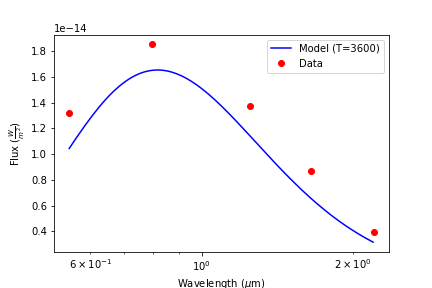
\includegraphics [scale=0.9] {prob3}

\end{document}
